\section{Conclusion} \label{sec:conclusion}
We showed that conventional CNN architectures can be used to generate 3D shapes as point clouds once they are ordered using kd-trees.
We found that a hundred linear basis are generally sufficient to model a category of diverse shapes such as chairs.
By employing GANs to model the multi-modal distribution of the basis coefficients we showed that our method outperforms the PPCA baseline approach.
The ordering of points produced by the kd-tree also allows reasonable shape generation using 1D-GANs.
Our approach is of comparable quality but considerably more lightweight than 3D voxel-based shape generators.
Moreover it allows the incorporation of multiple point attributes such normals and color in a seamless manner.
In the next chapter, we further investigate the role of space-partitioning data structures on 3D shape classification and segmentation tasks.
We also explore incorporating permutation invariant losses in conjunction with multi-grid architectures
for unconditional shape generation and reconstruction from single RGB images.
\begin{figure}[h]
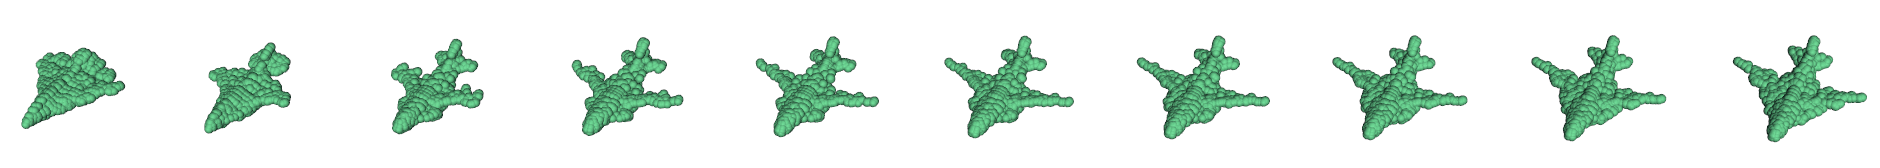
\includegraphics[width=1.0\linewidth]{PCAGAN/images/airplane_interpolation2.png}
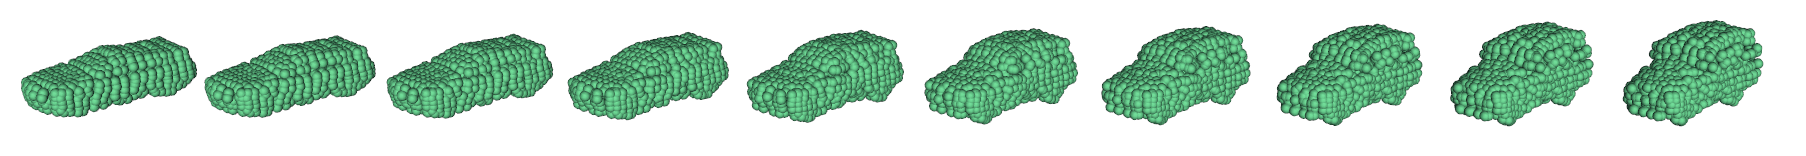
\includegraphics[width=1.0\linewidth]{PCAGAN/images/car_interpolation2.png}
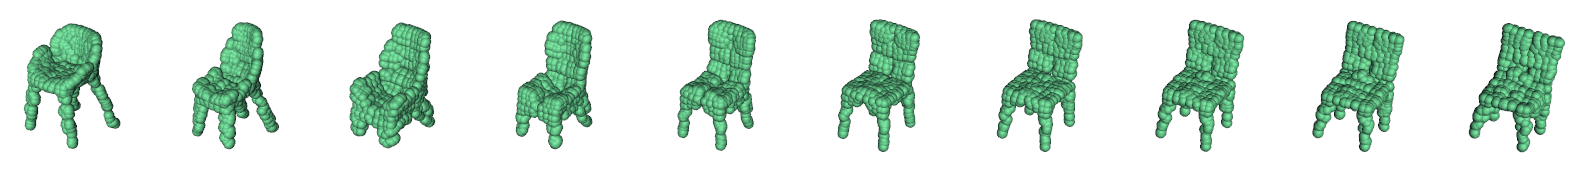
\includegraphics[width=1.0\linewidth]{PCAGAN/images/chair_interpolation2.png}
\vspace{-16pt}
\caption{\small \label{pca:interpolation} Interpolation of the encodings $z$ between a start shape and an end shape for each of the three categories shown here: airplane, car, and chair.}
\vspace{-12pt}
\end{figure}
